\documentclass{standalone}

\usepackage{pgf}
\usepackage{tikz}
\usetikzlibrary{arrows,automata,matrix}
\usepackage[latin1]{inputenc}
\begin{document}
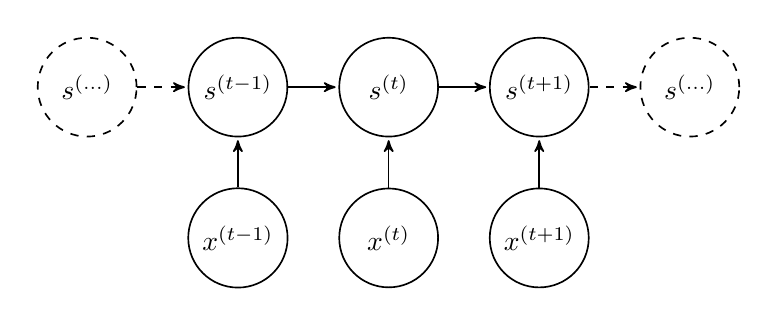
\begin{tikzpicture}[->,>=stealth'
  ,shorten >=1pt
  ,auto
  ,node distance=2.8cm,
  semithick]
  \tikzstyle{every state}=[minimum size={10pt+width("$x^{(t-1)}$")}]

  \matrix (m) [matrix of nodes
  ,row sep=.25in,column sep=.25in]
  {
    % 5 s's top row
    \node[state,dashed](sd) {$s^{(\ldots)}$};	&
    \node[state](stm1) {$s^{(t-1)}$};	 	&
    \node[state](st) {$s^{(t)}$}; 		&
    \node[state](stp1) {$s^{(t+1)}$};		&
    \node[state,dashed](sd2) {$s^{(\ldots)}$}; 	\\
    % 3 xs btm
    &
    \node[state](xtm1) {$x^{(t-1)}$}; 		&
    \node[state](xt) {$x^{(t)}$}; 		&
    \node[state](xtp1) {$x^{(t+1)}$} ;		\\
  };
  
  \path[dashed]  (sd) edge       node {} (stm1);
  \path 
  (xtm1) edge  node {} (stm1)
  (stm1) edge       node {} (st)
  (xt) edge  node {} (st)
  (st) edge       node {} (stp1)
  (xtp1) edge  node {} (stp1);
  \path[dashed] (stp1) edge       node {} (sd2)
  ;
  
\end{tikzpicture}

\end{document}